% version 1.00	date 29/01/2016  	Auteur Pierre Porche

\section*{Informations générales}
 
\begin{table}[h]
\centering
	\begin{tabularx}{16.8cm}{|X|X|}
	\hline
	\rowcolor{gray!40} Numéro du risque & Type du risque \\
	\hline
	003 & Absence collective \\
	\hline
	\end{tabularx}
\end{table}

\begin{table}[h]
\centering
	\begin{tabularx}{16.8cm}{|X|X|X|}
	\hline
	\rowcolor{gray!40} Date & Visa du \RQ & Visa du \CP \\
	\hline
	 27/01/16 & pgpic & pgpic \\
	\hline
	\end{tabularx}
\end{table}

\begin{table}[h]
\centering
	\begin{tabularx}{16.8cm}{|X|X|X|X|}
	\hline
	\rowcolor{gray!40} Pilote & Activité WBS & Compte WBS & Phase d'apparition \\
	\hline
	 \Pierre & Suivre les Risques et Opportunités & 1.2.3.2 & À partir du début du projet \\
	\hline
	\end{tabularx}
\end{table}

\section*{Description du risque}

\subsection*{Résumé}
	Le risque lié à une absence collective peut entraîner un ralentissement voire un arrêt total du travail et donc perturber grandement le planning.
	
\subsection*{Analyse des causes}
	voir figure \ref{risque absence collective}.

\subsection*{Criticité}

\begin{table}[h]
\centering
	\begin{tabularx}{12.8cm}{|>{}X|X|}
	\hline
	Gravité & 4\\
	\hline
	Probabilité & 1\\
	\hline
	Criticité & Critique\\
	\hline
	\end{tabularx}
\end{table}
\newpage

\section*{Actions}
\subsection*{Actions préventives}

%\begin{table}[H]
\centering
	\begin{longtable}{|p{7cm}|p{7cm}|}
	\hline
	\rowcolor{gray!40} Numéro de cause & Actions préventives \\
	\hline
	 1 & \begin{itemize}
	 	\item Prévenir en cas de maladie
	 	\item Le \CP{} doit se tenir au courant des épidémies en temps réel
	 \end{itemize} \\

	\hline
	2 & \begin{itemize}
		\item Avoir une bonne planification
	\end{itemize} \\
	\hline
	3 & \begin{itemize}
		\item Se tenir au courant des faits d'actualité
	\end{itemize} \\
	\hline
	\end{longtable}
%\end{table}

\flushleft
\subsection*{Plan de contournement}

\begin{enumerate}
	\item Résumer l'état des présences de chacun.
	\item Prévenir le client ainsi que le tuteur pédagogique.
	\item Réorganiser le planning de manière à avoir une perte de productivité la moins importante possible.
	\item Réorganiser le planning de nouveau dès le retour des absents.
\end{enumerate}

\section*{Décision de clôture}
Par le \CP{} et le pilote du risque.
\begin{table}[H]
\centering
	\begin{tabularx}{12.8cm}{|X|X|}
	\hline
	\rowcolor{gray!40} Date de clôture & Raison de la clôture \\
	\hline
	  & \\
	\hline
	\end{tabularx}
\end{table}

\section*{Historique des modifications}
\begin{table}[H]
\centering
	\begin{tabularx}{12.8cm}{|X|X|}
	\hline
	\rowcolor{gray!40} Date & Modification \\
	\hline
	  & \\
	\hline
	\end{tabularx}
\end{table}
\newpage


\begin{figure}
	\centering
	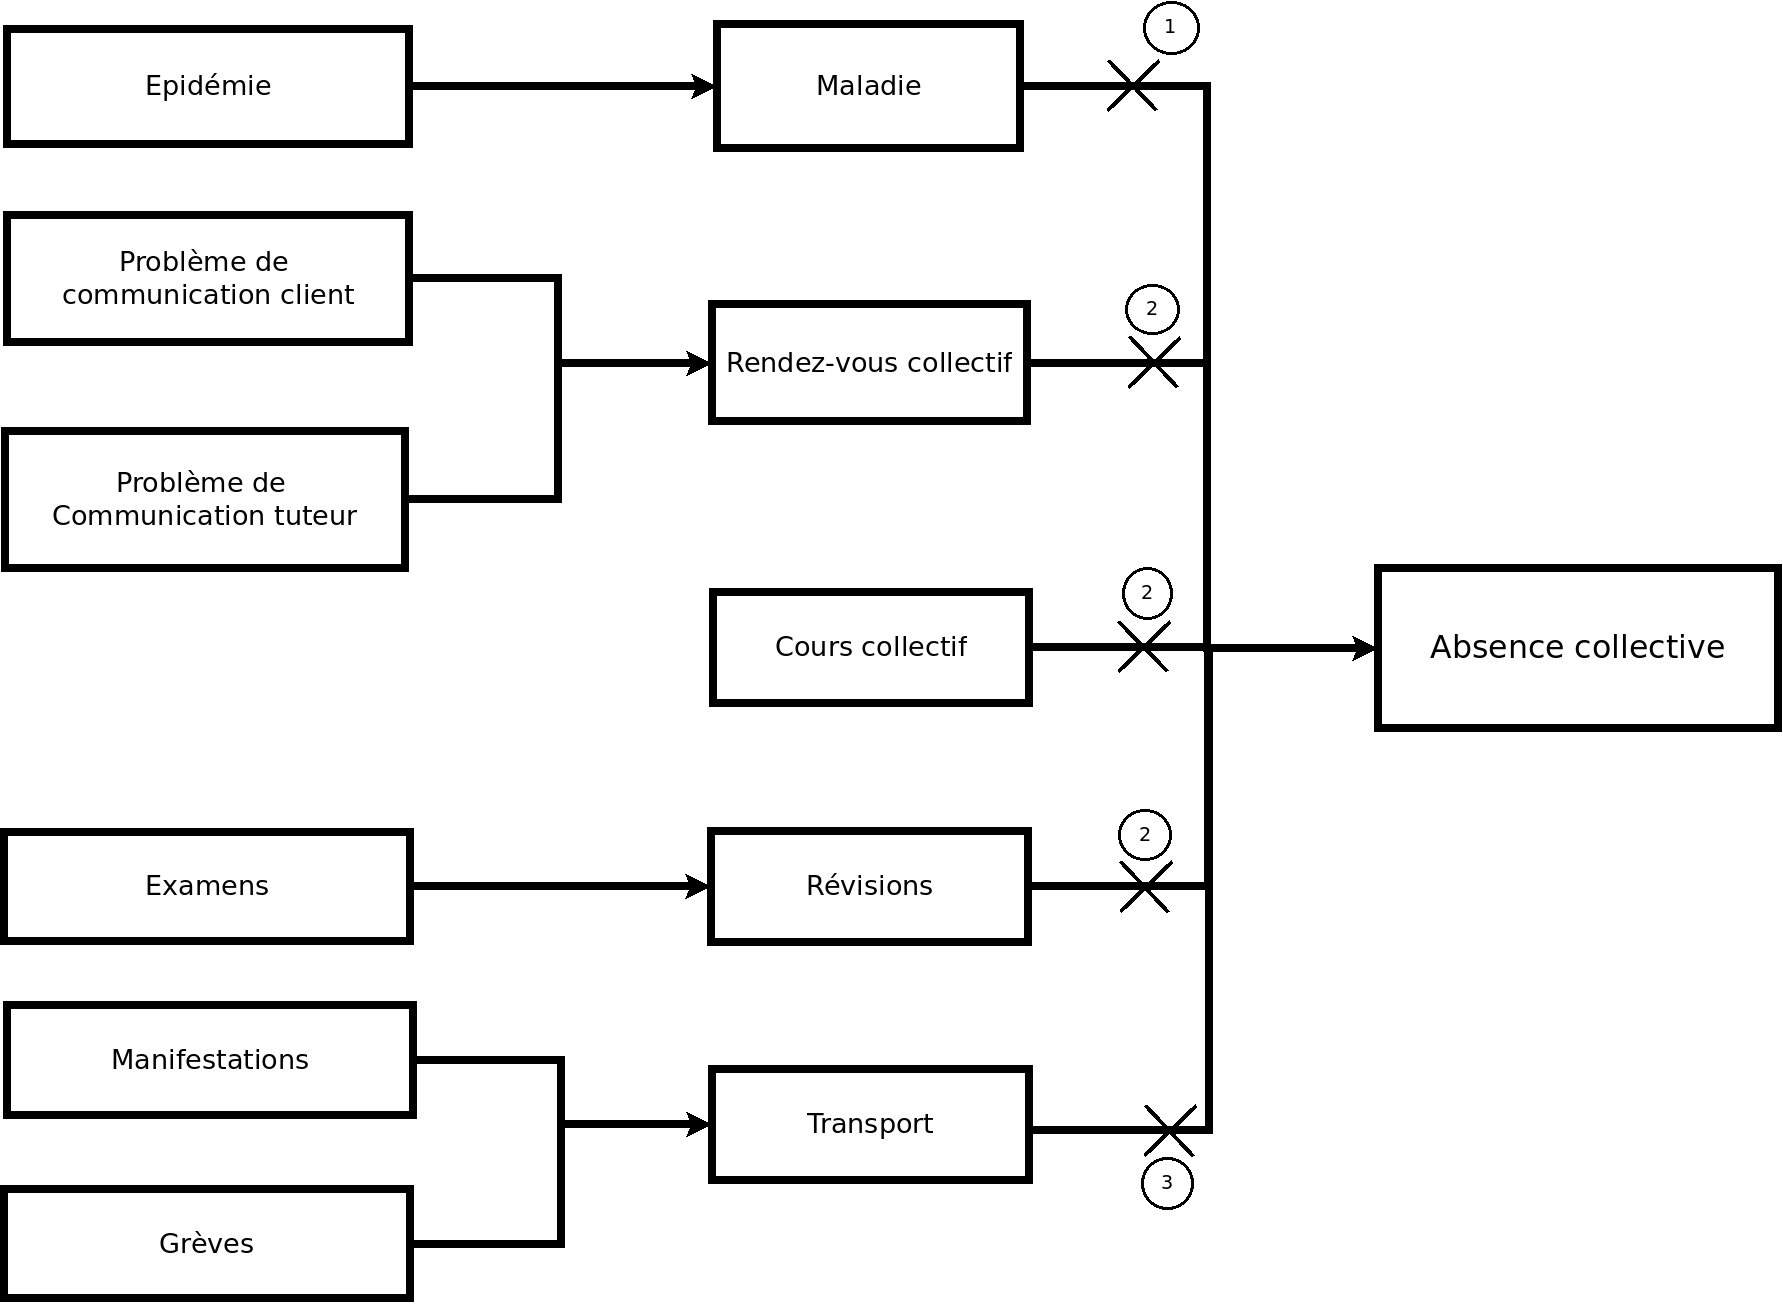
\includegraphics[scale=0.2]{images/AnalyseRisque_nPourquoi_FDR003}
        \caption{\label{risque absence collective}risque absence collective - méthode des n pourquoi}
\end{figure}
